\section{Результаты}
Для замеров скорости работы программы на $CPU$ мною была написана программа, создающая множество потоков, каждый из них обрабатывает входные векторы, начиная с определенного индекса и с шагом, равным количеству векторов.
Так как каждый поток только считывает данные из входных векторов, то необязательно их защищать от гонки потоков. Также каждый индекс обрабатывается только одним потоком, поэтому защищать результат от гонки потоков тоже необязательно с целью повышения производительности программы.

В замер времени работы программмы входит промежуток от создания потока до завершения работы всех потоков (метод $join()$ для каждого потока). Общее количество потоков ограничено сверху значением $1000$. Также стоит отметить, что время выполнения работы сильно связано с загрузкой системы и с самой системой, так как создание потока - блокирующий системный вызов.

Замеры времени работы обоих программ проходили на одинаковых тестах. В качестве входных чисел были использованы псевдослучайные числа $c: -10^{10} \leq c \leq 10^{10}$

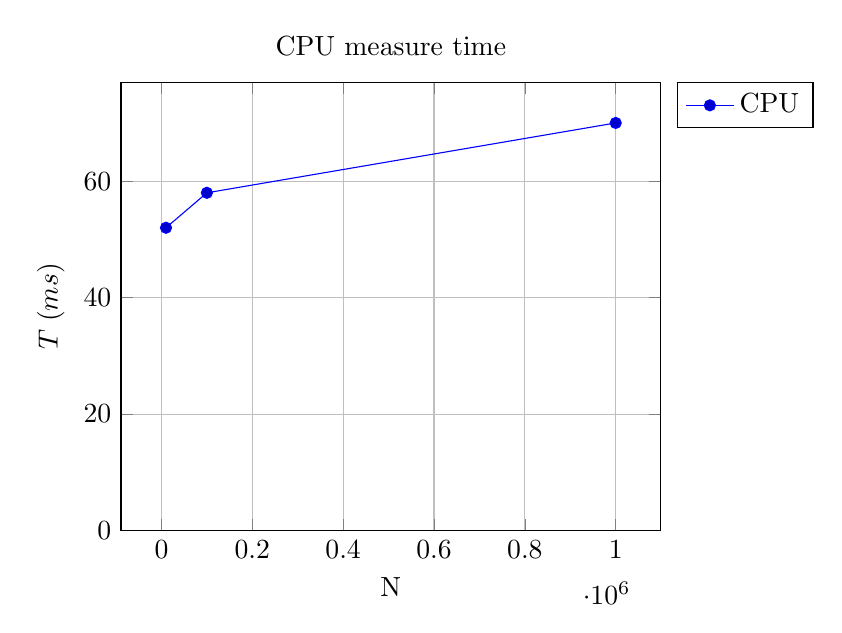
\begin{tikzpicture}% coordinates
	\begin{axis}[
		title = CPU measure time,
		xlabel=N,
		ylabel= $T\;(ms)$,
		ymin = 0,
		grid=major,
		legend pos = outer north east
		]
		\legend{CPU}
		\addplot coordinates {(10000, 52.0) (100000, 58.0) (1000000, 70.0)};
	\end{axis}
\end{tikzpicture}

По графику видно, что создание потоков на $CPU$ и ожидание их выполнения происходит достаточно долго.

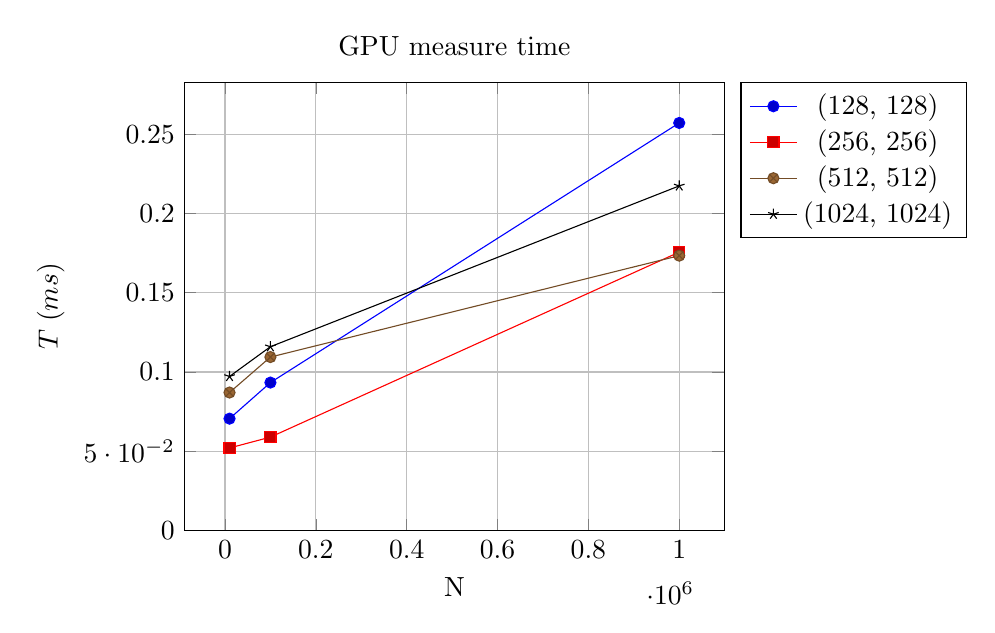
\begin{tikzpicture}% coordinates
	\begin{axis}[
		title = GPU measure time,
		xlabel=N,
		ylabel= $T\; (ms)$,
		ymin = 0,
		grid=major,
		legend pos = outer north east
		]
		\legend{(128, 128), (256, 256), (512, 512), (1024, 1024)}
		\addplot coordinates {(10000, 0.07056) (100000, 0.093312) (1000000, 0.257088)};
		\addplot coordinates {(10000, 0.052064) (100000, 0.058912) (1000000, 0.175616)};
		\addplot coordinates {(10000, 0.08704) (100000, 0.109408) (1000000, 0.173376)};
		\addplot coordinates {(10000, 0.097184) (100000, 0.115936) (1000000, 0.217376)};
	\end{axis}
\end{tikzpicture}

В то же время исполнение программы на $GPU$ происходит гораздо быстрее. Это связано с легковесностью потоков на $GPU$, а также с гораздо б\'oльшим количеством потоков, исполняющихся одновременно.
Также из графика можно заключить, что оптимальной конфигурацией для данного оборудования будет $<<< 256, 256 >>>$. Также видно, что на маленьких данных конфигурации с маленькими значениями выигрывают конфигурации с большими значениями, так как сказывается процесс создания потоков.